%=======================================================================
%  ÖZET RAPOR — yöntem envanteri + sonuçlar, haberleşme odaklı
%  Derleme: xelatex ozet_rapor.tex (iki kez)
%=======================================================================
\documentclass[11pt,a4paper]{article}

\usepackage{fontspec}
\setmainfont{Cambria}
\setsansfont{Calibri}
\setmonofont{Consolas}[Scale=0.86]

\usepackage[shorthands=off,turkish]{babel}
\usepackage[a4paper,margin=2.1cm,top=2.2cm,bottom=2.2cm]{geometry}
\usepackage{booktabs}
\usepackage{longtable}
\usepackage{array}
\usepackage{graphicx}
\usepackage{xcolor}
\usepackage{amsmath}
\usepackage{enumitem}
\usepackage{float}
\usepackage{caption}
\usepackage{fancyhdr}
\usepackage{tcolorbox}
\usepackage[hidelinks]{hyperref}

\tcbuselibrary{skins,breakable}

\definecolor{anaRenk}{HTML}{1F4E79}
\definecolor{uyariRenk}{HTML}{9C2B00}
\definecolor{acikGri}{HTML}{F2F4F7}
\definecolor{acikMavi}{HTML}{EAF1F8}
\definecolor{acikSari}{HTML}{FDF3E3}

\captionsetup{font=small,labelfont={bf,color=anaRenk}}
\setlength{\parskip}{0.40em}
\setlength{\parindent}{0pt}
\renewcommand{\arraystretch}{1.14}
\tolerance=1800
\emergencystretch=4em
\hbadness=10000

\renewcommand{\tablename}{Çizelge}
\renewcommand{\figurename}{Şekil}
\renewcommand{\contentsname}{İçindekiler}

\pagestyle{fancy}
\fancyhf{}
\fancyhead[L]{\footnotesize\sffamily\color{anaRenk}Açıklanabilirliğin Maliyeti --- Özet Rapor}
\fancyhead[R]{\footnotesize\sffamily\thepage}
\renewcommand{\headrulewidth}{0.4pt}

\newtcolorbox{bulgu}[1][]{breakable,enhanced,colback=acikMavi,colframe=anaRenk,
  boxrule=0.8pt,left=8pt,right=8pt,top=6pt,bottom=6pt,
  fonttitle=\bfseries\sffamily\small,title={#1}}
\newtcolorbox{uyari}[1][Uyarı]{breakable,enhanced,colback=acikSari,colframe=uyariRenk,
  boxrule=0.8pt,left=8pt,right=8pt,top=6pt,bottom=6pt,
  fonttitle=\bfseries\sffamily\small,title={#1}}
\newtcolorbox{tanim}[1][]{breakable,enhanced,colback=acikGri,colframe=black!25,
  boxrule=0.5pt,left=8pt,right=8pt,top=6pt,bottom=6pt,
  fonttitle=\bfseries\sffamily\small,title={#1}}

\newcommand{\ms}{\,ms}
\newcommand{\kod}[1]{\texttt{\small #1}}
\newcommand{\dosya}[1]{\texttt{\footnotesize #1}}

\begin{document}

%-----------------------------------------------------------------------
\begin{center}
{\sffamily\small\color{anaRenk} ÖZET RAPOR \quad·\quad 28 Eylül 2026}\\[0.5em]
{\sffamily\LARGE\bfseries\color{anaRenk} Gerçek Zamanlı Stres Tespitinde\\[0.15em]
Açıklanabilirliğin Hesaplama Maliyeti}\\[0.45em]
{\sffamily\large Yöntem Envanteri ve Ölçüm Sonuçları}
\end{center}

\vspace{0.3em}
\begin{tcolorbox}[colback=acikMavi,colframe=anaRenk,boxrule=1pt,
  left=10pt,right=10pt,top=8pt,bottom=8pt]
\sffamily\small
\textbf{Bu rapor kimin için.} Makine öğrenmesi ve XAI kavramlarını bildiğin
varsayılıyor --- SHAP, LIME, faithfulness, ECE gibi terimler tanımlanmıyor,
yalnızca \emph{hangi varyantı, hangi ayarla} kullandığımız yazılıyor. Buna
karşılık \textbf{haberleşme ve dağıtık sistem tarafı} (Bölüm~3) ayrıntılı
anlatılıyor, çünkü işin yeni olduğun kısmı orası.

\vspace{0.25em}
\textbf{Yapı.} Bölüm~2 projede kullanılan \emph{bütün} yöntemlerin envanteri;
Bölüm~3 haberleşme altyapısı ve yedi metrik; Bölüm~4 sonuçlar; Bölüm~5
uyarılar. Her yöntem yalnızca bir yerde anlatılır, sonuç bölümünde tekrar
edilmez.

\vspace{0.25em}
\textbf{Ayrıntılı sürüm.} Her deneyin tam dökümü, tam sözlük, geçersiz sayılan
ölçümlerin gerekçeleri ve bitirme projesi sonuçları:
\dosya{docs/teknik\_rapor.pdf} (53 sayfa). Bütün sayılar aynı kaynaklardan
gelir.
\end{tcolorbox}

%=======================================================================
\section{Ana bulgular}

\begin{bulgu}[Tek cümlelik sonuç]
Gerçek zamanlı bir stres tespit sisteminde darboğaz \textbf{tahmin değil,
açıklamadır}. Sis düğümünde bir 10 saniyelik pencerenin tahmini 3{,}39\ms,
aynı pencerenin SHAP/LIME açıklaması 395--1422\ms{} sürüyor --- toplam hesabı
\textbf{118--421 kat} büyütüyor. Bunun sonucu: sistem tasarımındaki kritik
karar \emph{``hesabı nerede yapayım''} (uç/sis/bulut) olmaktan çıkıp
\emph{``ne zaman açıklayayım''} olmaya kayıyor.
\end{bulgu}

\begin{table}[H]
\centering\small
\begin{tabular}{@{}p{7.6cm}rl@{}}
\toprule
\textbf{Bulgu} & \textbf{Sayı} & \textbf{Kaynak} \\
\midrule
Açıklamanın toplam hesabı büyütme oranı & 118--421$\times$ & \dosya{04\_fog/} \\
Yerleşim farkı, açıklama \emph{kapalıyken} (bulut/uç) & 8{,}7$\times$ & \dosya{13\_bulut/} \\
Yerleşim farkı, açıklama \emph{açıkken} (bulut/uç, SHAP) & \textbf{1{,}13$\times$} & \dosya{13\_bulut/} \\
Seçici açıklamanın ortalama yanıtta kazancı & 5{,}6$\times$ & \dosya{09\_secici\_xai/} \\
Seçici açıklamanın kapasitede kazancı & 7{,}5$\times$ & \dosya{10\_yuk/} \\
Projeksiyon ile ölçümün uyumu & \%2 & \dosya{09\_secici\_xai/} \\
\bottomrule
\end{tabular}
\end{table}

\begin{bulgu}[Önerilen çözüm ve ölçülen kazancı]
\textbf{Güven eşikli seçici açıklama:} model kendinden eminse (güven $\geq$
0{,}80) sadece tahmin döndür; emin değilse tahmin + açıklama döndür.
\textbf{1030 pencerelik} gerçek bir koşuda ölçüldü: ortalama yanıt süresi
$450{,}5 \rightarrow 80{,}1$\ms{} (\textbf{5{,}6$\times$}), pencerelerin
yalnızca \textbf{\%14{,}1}'i açıklanıyor, buna rağmen yanlış sınıflanan
pencerelerin \textbf{\%89{,}7}'si açıklama alıyor, tek işçili kapasite
$12 \rightarrow 90$ eşzamanlı istemci.
\end{bulgu}

%=======================================================================
\section{Kullanılan yöntemler envanteri}

Bu bölüm ``projede ne yaptık'' sorusunun tam cevabıdır. Her satır: yöntem,
nerede kullanıldığı, ve varsa ölçülen değeri.

%-----------------------------------------------------------------------
\subsection{Veri ve sinyal işleme}

\begin{longtable}{@{}p{4.0cm}p{2.9cm}p{8.6cm}@{}}
\toprule
\textbf{Yöntem} & \textbf{Nerede} & \textbf{Ne yapıldı / ölçüldü} \\
\midrule
\endfirsthead
\toprule
\textbf{Yöntem} & \textbf{Nerede} & \textbf{Ne yapıldı / ölçüldü} \\
\midrule
\endhead
Çok kanallı birleştirme & \dosya{data/loader.py} &
Göğüs 8 + bilek 6 = 14 kanal. \textbf{Sabit sıra zorunlu}: sıra bozulunca
doğruluk 1{,}00'den 0{,}52'ye düştü (gözlendi). \\
\addlinespace
Ham hızda (native) akış & \kod{NATIVE\_STREAMS} &
Göğüs 700\,Hz; bilek ACC 32\,Hz, BVP 64\,Hz, EDA/TEMP 4\,Hz. Her akış kendi
hızında taşınır. \\
\addlinespace
Doğrusal interpolasyonla yeniden örnekleme & \kod{np.interp} &
Hepsi ortak 64\,Hz'e indirilir. \textbf{Pencere başına, sunucuda} yapılır, yani
maliyeti ölçülür: \textbf{1{,}57\ms{} = toplamın \%28{,}6'sı}. \\
\addlinespace
Kayan pencere & \kod{MultiRateBuffer} &
10\,s = 640 örnek, hop 5\,s = 320 örnek, \textbf{\%50 örtüşme} $\rightarrow$
her 5 saniyede bir yeni tahmin. \\
\addlinespace
İki tampon stratejisi & \dosya{streaming/buffer.py} &
\kod{RollingBuffer} (indirgeme ölçüm dışında) ile \kod{MultiRateBuffer}
(indirgeme ölçüm içinde) karşılaştırıldı. \\
\addlinespace
Tick tabanlı replay & \dosya{streaming/} &
500\ms'lik bloklar hâlinde gerçek zamanlı sensör akışı taklidi. \\
\addlinespace
Çoğunluk etiketi & pencereleme &
Geçersiz etiketli pencereler \textbf{işlenir} ama rapordan çıkarılır. Eskiden
atlanıyordu; bu normalizasyon istatistiğini bozuyordu, düzeltilince doğruluk
0{,}7674 $\rightarrow$ \textbf{0{,}8222}. \\
\addlinespace
İkili etiketleme & \kod{config} &
Stres (2) ile stres-değil (1, 3, 4: taban çizgi, eğlence, meditasyon). \\
\addlinespace
Alt-örnekleme & \dosya{data/windowing.py} &
Yalnızca offline eğitimde, sınıf dengesi için. \\
\bottomrule
\end{longtable}

%-----------------------------------------------------------------------
\subsection{Model ve eğitim}

\begin{longtable}{@{}p{4.0cm}p{2.9cm}p{8.6cm}@{}}
\toprule
\textbf{Yöntem} & \textbf{Nerede} & \textbf{Detay} \\
\midrule
\endhead
1B Temporal CNN & \dosya{models/}\newline\dosya{temporal\_cnn.py} &
Conv1d $\rightarrow$ BatchNorm $\rightarrow$ ReLU $\rightarrow$ MaxPool(2)
$\rightarrow$ Dropout, iki blok; sonra GAP $\rightarrow$ FC(128$\to$64)
$\rightarrow$ BN $\rightarrow$ ReLU $\rightarrow$ Dropout $\rightarrow$ FC(64$\to$2). \\
\addlinespace
Mimari seçimi & depth 2, [32,128], k9 &
\textbf{49\,890 parametre}, 14{,}50M MAC/pencere, tepe aktivasyon 81\,920
eleman (\kod{bn2}). \\
\addlinespace
Focal loss & eğitim & $\alpha=0{,}5$, $\gamma=2$ --- sınıf dengesizliği için. \\
\addlinespace
Adam + weight decay & eğitim & lr 1e-3, wd 1e-4, batch 64. \\
\addlinespace
Erken durdurma & eğitim & 150 epoch üst sınır, patience 20, seed 42. \\
\addlinespace
LOSO protokolü & değerlendirme &
15 katlı. Kanonik sayı \textbf{F1 0{,}92--0{,}93}. (Checkpoint'teki 0{,}9386
yalnızca iki denek üzerinde ve LOSO değil --- makalede kullanılmamalı.) \\
\addlinespace
Karşılaştırma modeli & \dosya{Transformer.ipynb} &
TranSenseFusers: Temporal CNN + 8 başlı çapraz dikkat (dim 64),
\textbf{1\,859\,026 param, 103{,}7\ms{} çıkarım} $\rightarrow$ CNN'e göre
37{,}3$\times$ parametre, 28{,}6$\times$ çıkarım. \\
\addlinespace
Checkpoint'ten mimari okuma & \kod{load\_checkpoint()} &
Mimari config'ten değil checkpoint'in kendi meta alanından okunur ---
sessiz mimari uyuşmazlığı imkânsız (\kod{strict=True}). \\
\bottomrule
\end{longtable}

\begin{uyari}[Model seçiminin gerekçesi ve iki dürüstlük notu]
Bitirmede en yüksek doğruluğu TranSenseFusers verdi (\%91{,}13) ama dağıtım
için 49{,}9K parametreli CNN donduruldu --- gerekçe gecikme.

\textbf{1.} \%91{,}13 \emph{LOSO değil}: tek test deneği (S3), doğrulama S16
(F1 1{,}0000). Makalede bu sayıya ``LOSO'' denmemeli.
\textbf{2.} Pencere hızı da farklı: transformer 700\,Hz'de 7000 örnek, CNN
64\,Hz'de 640 örnek --- 28{,}6$\times$ farkın bir kısmı buradan geliyor,
tabloda ``sampling rate'' sütunuyla gösterilmeli.
\end{uyari}

%-----------------------------------------------------------------------
\subsection{Normalizasyon}

\begin{longtable}{@{}p{4.0cm}p{2.9cm}p{8.6cm}@{}}
\toprule
\textbf{Yöntem} & \textbf{Kullanım} & \textbf{Ölçülen} \\
\midrule
\endhead
Denek bazlı z-score & offline eğitim &
Referans. Gerçek zamanlıda \textbf{kullanılamaz} --- geleceğe sızma. \\
\addlinespace
Nedensel z-score (Welford) & \kod{running}, \textbf{varsayılan} &
Sadece o ana kadarki veriden çevrimiçi ortalama/std. Güncelleme maliyeti
dürüstlük için \kod{preprocessing}'e eklenir (\textbf{0{,}25\ms}). \\
\addlinespace
Sabit z-score & \kod{fixed} &
Yalnızca eğitim deneklerinden tek bir mean/std; en katı dağıtım senaryosu. \\
\addlinespace
Sızıntı miktarının ölçümü & doğrulama &
İki girdi uzayı arasında bağıl L2 farkı \textbf{0{,}787 (S11) / 0{,}773 (S2)},
standart sapma 1{,}00'e karşı 1{,}25. \\
\bottomrule
\end{longtable}

\textbf{Ölçülen bedel:} offline weighted F1 0{,}9386 $\rightarrow$ streaming
doğruluk 0{,}8222. Düşüş modelin değil, \emph{normalizasyon kısıtının} sonucu
--- makalede bu cümle olmalı.

%-----------------------------------------------------------------------
\subsection{Açıklanabilirlik yöntemleri}

\begin{longtable}{@{}p{4.0cm}p{2.9cm}p{8.6cm}@{}}
\toprule
\textbf{Yöntem} & \textbf{Nerede} & \textbf{Detay} \\
\midrule
\endfirsthead
\toprule
\textbf{Yöntem} & \textbf{Nerede} & \textbf{Detay} \\
\midrule
\endhead
SHAP \textbf{GradientExplainer} & \dosya{xai/shap\_.py} &
Gradyan tabanlı, modelin içine erişir. \textbf{KernelSHAP değil} ---
literatürdeki ``SHAP yavaştır'' iddiası ona aittir, bizim sayılarımıza değil. \\
\addlinespace
k-means ile arka plan seçimi & \dosya{xai/artifacts.py} &
2355 pencerelik havuzdan \textbf{100 pencere}, S2--S5'ten (test denekleriyle
kesişmiyor), seed 42, nedensel uzayda. \\
\addlinespace
Arka planın dondurulması & \kod{.npz} + \kod{xai\_config.json} &
Diskten okunur ve \textbf{SHA-256 doğrulanır}. Sunucu her açılışta yeniden
kümelemez; tarama ile bit-birebir aynı sonuç garanti. \\
\addlinespace
\kod{nsamples} çalışma noktası & SHAP & 200 (tam) ve \textbf{50} (ucuz). \\
\addlinespace
\textbf{Bölge tabanlı LIME} & \dosya{xai/lime\_.py} &
Hazır \kod{lime} paketi \textbf{kullanılmadı}. Görüntüdeki süper-pikselin
karşılığı: 20 zaman dilimi $\times$ 14 kanal = \textbf{280 bölge}. \\
\addlinespace
Rastgele ikili maske örnekleme & LIME &
250 / 500 perturbasyon, seed sabit; ilk örnek hep orijinal pencere. \\
\addlinespace
Kanal ortalamasıyla maskeleme & LIME + kalite metrikleri &
Sıfırlamak yerine. Normalize sinyalde sıfır ``bilgi yok'' değil ``kaydın
ortalaması'' demektir ve fizyolojik olarak anlamsızdır. \\
\addlinespace
Üstel kernel ağırlıklandırma & LIME &
$w=\sqrt{\exp(-d^2/kw^2)}$, $kw=0{,}5$; $d$ = kapalı bölge oranı. \\
\addlinespace
Ağırlıklı Ridge regresyon & LIME &
$\alpha=1{,}0$; katsayılar doğrudan atıf haritası olur. \\
\addlinespace
Partili ileri geçiş & \dosya{xai/base.py} &
chunk 256. \kod{model.eval()} olduğu için parti boyutu sonucu değiştirmez ---
BatchNorm koşu istatistiklerini kullanır. \\
\addlinespace
Bölge ızgarası önbellekleme & LIME &
Her çağrıda yeniden kurmak, ölçülen gecikmeye modelin işi olmayan bir maliyet
eklerdi. \\
\addlinespace
Açıklayıcı ısıtma (warm-up) & \dosya{serving/server.py} &
SHAP \textbf{ilk} çağrı 12{,}4\,s, sonraki 0{,}85\,s. Isıtılmasa tek worker'ı
12 saniye bloklar, bütün kuyruk arkasında birikirdi. Ölçülen ısınma:
1208--1251\ms. \\
\addlinespace
\textbf{Seed sabitleme} & her iki yöntem &
Sabitlenmeden önce SHAP sensitivity 0{,}139'du, sonra \textbf{0{,}075} ---
farkın neredeyse yarısı yöntemin kendi gürültüsüymüş. \\
\addlinespace
OFAT taraması & Colab / GPU,\newline \dosya{wesad\_xai\_ofat\_}\newline\dosya{sweep\_colab.py} &
Her aşamada tek parametre değiştirilir: LIME 9 yapılandırma (örnek sayısı,
bölge sayısı, kernel genişliği), SHAP 8 (arka plan boyutu, \kod{nsamples},
seçim yöntemi). Colab/GPU, 40 pencere, nedensel uzay. \\
\bottomrule
\end{longtable}

\begin{table}[H]
\centering\small
\begin{tabular}{@{}llr@{}}
\toprule
\textbf{Çalışma noktası} & \textbf{Yapılandırma} & \textbf{Sis düğümünde} \\
\midrule
\kod{shap\_cheap} & GradientExplainer, arka plan 100 (kmeans), nsamples 50 & 395\ms \\
\kod{lime\_cheap} & bölge tabanlı, 280 bölge, 250 örnek, kw 0{,}5 & 590\ms \\
\kod{lime}        & aynı, 500 örnek & 1189\ms \\
\kod{shap}        & aynı, nsamples 200 & 1422\ms \\
\bottomrule
\end{tabular}
\caption{Taramadan \textbf{elle} seçilen dört çalışma noktası. Otomatik seçim
yalnızca faithfulness'a baktığı için kullanılmadı --- gerekçesi
\dosya{xai\_config.json}'a yazıldı.}
\end{table}

%-----------------------------------------------------------------------
\subsection{Açıklama kalitesi ölçütleri}

\begin{longtable}{@{}p{3.4cm}p{6.0cm}p{6.1cm}@{}}
\toprule
\textbf{Ölçüt} & \textbf{Nasıl hesaplanıyor} & \textbf{Ölçülen} \\
\midrule
\endhead
Deletion eğrisi + AUC & En önemliden başlayarak kapat, olasılığı izle; 20
kontrol noktası, trapez integral & Düşük AUC iyi \\
\addlinespace
Insertion eğrisi + AUC & Taban çizgiden başlayıp en önemliyi ekle & Yüksek AUC iyi \\
\addlinespace
\textbf{Faithfulness} & insertion AUC $-$ deletion AUC &
\textbf{0{,}209--0{,}263} --- dört nokta arasında \textbf{fark yok}
(SEM $\approx$0{,}04) \\
\addlinespace
Monotonicity & Insertion'da azalmayan adım oranı (yüksek iyi) & 0{,}549--0{,}604 \\
\addlinespace
\textbf{Sensitivity} & Gürültüye karşı normalize L2 değişim
($0{,}05\times\sigma$, 3 deneme, düşük iyi) &
LIME \textbf{0{,}045--0{,}049} vs SHAP \textbf{0{,}123--0{,}128} $\rightarrow$
LIME 2{,}7$\times$ kararlı, fark hata payının 15 katı \\
\addlinespace
Self-instability & Aynı pencere iki kez açıklanınca fark & Seed sabitken
$\approx$0, her iki yöntemde \\
\addlinespace
Kanal ortalaması taban çizgi & Ölçüt ile yöntem tutarlı olsun diye
açıklayıcıların kendi perturbasyonuyla aynı & --- \\
\addlinespace
\textbf{SEM} & $\sigma/\sqrt{n}$, $n=40$ pencere &
Taramanın ilk hâlinde \textbf{yoktu}; kazananlar 0{,}003'lük farkla
seçiliyordu. Eklenince o seçimin geçersiz olduğu anlaşıldı. \\
\addlinespace
Pareto analizi & \dosya{tools/pareto.py} & Kalite bu makinede (donanımdan
bağımsız), gecikme sis düğümünden (dağıtım donanımı) \\
\bottomrule
\end{longtable}

%-----------------------------------------------------------------------
\subsection{Güven kalibrasyonu}

\begin{longtable}{@{}p{4.0cm}p{4.0cm}p{7.5cm}@{}}
\toprule
\textbf{Yöntem} & \textbf{Nasıl} & \textbf{Sonuç} \\
\midrule
\endhead
Reliability diyagramı & 15 eşit genişlikli kutu & Şekil~\ref{fig:kal} \\
\addlinespace
ECE / MCE & Kutu ağırlıklı ve en büyük |güven $-$ doğruluk| &
S11 \textbf{0{,}047} / 0{,}252 · S14 \textbf{0{,}227} / 0{,}522 \\
\addlinespace
Brier / NLL & Olasılık tahmininin kare hatası / log kaybı &
S11 0{,}038 / 0{,}138 · S14 0{,}266 / 0{,}898 \\
\addlinespace
Fazla özgüven & ortalama güven $-$ doğruluk & S11 $-$0{,}043 · S14 \textbf{$+$0{,}218} \\
\addlinespace
Sıcaklık ölçekleme & NLL minimizasyonu ile tek parametre $T$ &
S11'de $T$=3{,}48, S14'te $T$=0{,}58 \\
\addlinespace
Çapraz denek uygulama & Bir denekte öğren, diğerinde uygula &
\textbf{Çalışmadı}: her iki yönde de kötüleştirdi \\
\addlinespace
Güven yüzdelikleri & p1, p5, p25, p50, p75, p95, p99 &
S11 p25 = 0{,}918 $\rightarrow$ düşük güven nadir; seçici açıklamanın kazancı
buradan gelir \\
\bottomrule
\end{longtable}

%-----------------------------------------------------------------------
\subsection{Seçici açıklama (ana katkı)}

\begin{longtable}{@{}p{4.0cm}p{11.5cm}@{}}
\toprule
\textbf{Yöntem} & \textbf{Detay} \\
\midrule
\endhead
Güven eşikli tetikleme & \kod{should\_explain(conf, $\tau$)}: \kod{conf $<$ $\tau$}
ise açıkla. $\tau$=0 hiç (XAI'siz taban), $\tau$=1 her pencere (en pahalı durum),
arası seçici. 1{,}0 ayrıca ele alınır çünkü softmax tam 1{,}0 okuyabiliyor. \\
\addlinespace
Aynı worker içinde üretim & Açıklama, tahminle aynı worker'da ve
\kod{execution time}'ın \emph{içinde} çalışır. Ayrı ipliğe atılsaydı maliyeti
görünmez olurdu --- deneyin bütün amacı o maliyeti ölçmek. \\
\addlinespace
Eşik taraması & 4 aday: 0{,}60 / 0{,}70 / 0{,}80 / 0{,}90, iki denekte. \\
\addlinespace
Üç karar ölçütü & \kod{explain\_rate} (maliyet), \kod{error\_recall} (fayda),
\kod{precision\_of\_trigger} (israf: açıklananların kaçı gerçekten hatalıydı). \\
\addlinespace
Karışım (mixture) modeli & $\text{ort} = (1-p)\cdot\text{taban} +
p\cdot\text{açıklamalı}$. 4 açıklayıcı $\times$ 2 denek $\times$ 6 eşik = 48
satırlık projeksiyon (\dosya{tools/selective\_sweep.py}). \\
\addlinespace
Projeksiyonun ölçümle sınanması & Ölçülen tek nokta ($\tau$=0{,}80, S11) ile
tahmin karşılaştırıldı $\rightarrow$ \textbf{\%2} uyum. \\
\bottomrule
\end{longtable}

%-----------------------------------------------------------------------
\subsection{Deney tasarımı ve ölçüm metodolojisi}

\begin{longtable}{@{}p{4.0cm}p{11.5cm}@{}}
\toprule
\textbf{Kural / yöntem} & \textbf{Gerekçe ve ölçülen} \\
\midrule
\endfirsthead
\toprule
\textbf{Kural / yöntem} & \textbf{Gerekçe ve ölçülen} \\
\midrule
\endhead
Isınma penceresi hariç & İlk \textbf{15} pencere hiçbir istatistiğe girmez
(önbellek/CUDA ısınması). \\
\addlinespace
\textbf{Dönüşümlü tekrar} & A, B, A, B sırası. Ardışık koşulsaydı işlemci
frekans ölçeklemesi son ölçülen yapılandırmayı sistematik olarak yavaş
gösterirdi. \\
\addlinespace
İki dağılımın ayrılması & \emph{Koşu içi} (bir koşudaki yüzlerce pencerenin
p50/p95/p99 --- sistemin davranışı) ile \emph{koşu arası yayılım} (aynı deney
tekrarlanınca medyanın oynaması --- ölçümün güven aralığı) karıştırılmaz. \\
\addlinespace
p50 / p95 / p99 birlikte & ``En hızlı çalışma'' hiçbir yerde raporlanmaz. \\
\addlinespace
\kod{range\_pct} ve CV & Yayılımın iki ölçüsü: (max$-$min)/medyan ve
$\sigma/\mu$. \\
\addlinespace
Tek iş parçacığı & 1/2/4 iplik, 4 tur dönüşümlü taranıp karar verildi. Fark
yayılımın altında kaldı; \textbf{gerekçe hız değil kararlılık}
(yayılım \%2{,}9'a karşı \%11--15). \\
\addlinespace
İki ardışık düzen yolu & \kod{prepared} (indirgeme ölçüm dışında) ile
\kod{native} (içinde) karşılaştırıldı; fark \%38{,}6, yayılımın (\%9{,}4) çok
üstünde, yani gerçek. \\
\addlinespace
Çapraz doğrulama denetimi & Tek süreçli yol ile istemci--sunucu yolu
\textbf{birebir aynı} sınıflandırma sonucunu veriyor (acc 0{,}8222,
TN 743 / FP 184 / FN 29 / TP 242) $\rightarrow$ ağ katmanı hesabı bozmuyor. \\
\addlinespace
Batch boyutu 1 & Gerçek kullanıcı tek pencere gönderir. \\
\addlinespace
Her sonuç JSON'a & Grafikler JSON'dan üretilir
(\kod{python -m tools.figures}); elle sayı taşınmaz. \\
\addlinespace
Koşu künyesi & Sunucu donanımı, Python/PyTorch sürümü, XAI yöntemi, eşik ve
tam yapılandırma her koşuya kaydedilir. \textbf{Yazılım yığını farkı bu sayede
yakalandı} (Bölüm~5). \\
\bottomrule
\end{longtable}

%-----------------------------------------------------------------------
\subsection{Donanım fizibilite analizi (ölçüm değil, hesap)}

\dosya{tools/mcu\_feasibility.py} modelin bir mikrodenetleyicide çalışıp
çalışmayacağını \emph{donanım olmadan} hesaplar.

\begin{table}[H]
\centering\small
\begin{tabular}{@{}p{4.6cm}p{10.4cm}@{}}
\toprule
\textbf{Yöntem} & \textbf{Sonuç} \\
\midrule
Katman katman parametre / aktivasyon / MAC sayımı & 49\,890 parametre,
14\,497\,984 MAC/pencere \\
Tepe aktivasyon analizi & 81\,920 eleman, \kod{bn2} katmanında ---
darboğaz orada (128 kanal $\times$ 320 uzunluk) \\
Nicemleme senaryoları & fp32 / fp16 / int8 $\rightarrow$ Flash 194{,}9 / 97{,}4 /
48{,}7\,KB; tepe RAM 320 / 160 / 80\,KB \\
MAC/çevrim tabanlı süre tahmini & Cortex-M4@168\,MHz 287{,}7\ms{} ·
M7@480\,MHz fp32 37{,}8\ms{} · M7 int8 12{,}1\ms{} --- en yavaşı bile
5000\ms{} bütçenin \%5{,}8'i \\
\midrule
\multicolumn{2}{@{}p{15cm}@{}}{\textbf{Sonuç:} MCU'da darboğaz hız değil
\textbf{bellek}. int8 nicemleme STM32F407/F746 için zorunlu; H743 ve U575
fp32'yi de kaldırır. \emph{Bu analiz kâğıt üstündedir} --- gerçek port ONNX
aktarımı, nicemleme, ön işleme portu ve cihaz üstü ölçüm gerektirir.} \\
\bottomrule
\end{tabular}
\end{table}

%-----------------------------------------------------------------------
\subsection{Bilinçli olarak kullanılmayanlar}

\begin{table}[H]
\centering\small
\begin{tabular}{@{}p{4.6cm}p{10.4cm}@{}}
\toprule
\textbf{Yöntem} & \textbf{Neden yok} \\
\midrule
KernelSHAP & GradientExplainer seçildi (gradyan erişimi var, çok daha hızlı).
Makalede açıkça yazılmalı, yoksa ``SHAP yavaş'' literatürüyle çelişik görünür. \\
Integrated Gradients & Bitirme projesinde vardı, bu çalışmanın kapsamı dışında. \\
Hazır \kod{lime} paketi & 8960 değişkeni ayrı ayrı saymak hem pahalı hem
yorumlanamaz. \\
Broker & Tek worker varken dağıtacak iş yok; referansın kendi sonucunda da
broker/worker farkı 43{,}9'a karşı 43{,}3\ms. \\
Çok worker & Tek worker varsayımı referansla aynı ve kuyruk metriğinin ön
koşulu. \\
Model karmaşıklığı ablasyonu & OFAT tablosu var ama varyantlar eğitilmedi ---
Kasım seti. \\
Kullanıcı çalışması & Standart XAI sınırlılığı. \\
\bottomrule
\end{tabular}
\end{table}

%=======================================================================
\section{Haberleşme tarafı: altyapı ve ölçüm yöntemleri}

Bu bölüm ölçümlerin \emph{neyi} ölçtüğünü anlatır. Sayılara geçmeden önce
okunması gereken kısım burasıdır.

\subsection{Üç yerleşim ne demek}

\begin{tanim}[Yerleşim (placement) --- hesabın fiziksel olarak nerede yapıldığı]
\begin{description}[leftmargin=0pt,style=nextline,itemsep=0.3em]
\item[Uç / ortak yerleşim (edge, co-located)] Sunucu, istemciyle
\textbf{aynı makinede}. Konuşma TCP \emph{loopback} (127.0.0.1) üzerinden:
gerçek ağ kartı ve kablo devrede değil, paket işletim sisteminin içinden döner.
Ağ gecikmesi $\approx$1\ms. \emph{Dikkat:} bu raporda ``edge'' \textbf{giyilebilir
cihaz anlamına gelmiyor}; makalede ``co-located'' demek daha güvenli.

\item[Sis (fog)] \textbf{Aynı yerel ağdaki ikinci fiziksel makine}
(192.168.1.14, Intel 12 çekirdek, 16\,GB), Wi-Fi üzerinden. Ağ gecikmesi
4--5\ms. Literatürde ``fog'' = kullanıcıya yakın, sınırlı kaynaklı sunucu
(tipik olarak Raspberry Pi). \emph{Buradaki makine güçlü olduğu için ölçülen
şey aslında ``dağıtık yerleşim'', ``kaynak kısıtlı sis düğümü'' değil} ---
Bölüm~5.

\item[Bulut (cloud)] İnternetteki uzak VPS (DigitalOcean, 167.71.43.64,
\textbf{1 çekirdek}, 2\,GB), Docker konteynerinde. Ağ gecikmesi 40--60\ms.
\end{description}
\end{tanim}

\subsection{Mimari ve üç tasarım kararı}

\begin{tcolorbox}[colback=acikGri,colframe=black!30,boxrule=0.6pt]
\ttfamily\footnotesize
İSTEMCİ (veri burada kalır --- sunucu WESAD'a ihtiyaç duymaz)\\
\hspace*{1em}her 500 ms'de bir "tick" bloğu $\rightarrow$ TCP paketi, t\_send damgası\\
\hspace*{2em}$\downarrow$\quad AĞ (loopback / Wi-Fi / internet)\\
SUNUCU — okuyucu görevi: paketi al, t\_recv damgala, KUYRUĞA koy\\
\hspace*{2em}$\downarrow$\quad (kuyrukta bekleme = queuing delay)\\
SUNUCU — TEK WORKER: t\_start $\rightarrow$ [resample $\rightarrow$ z-score\\
\hspace*{6em}$\rightarrow$ CNN $\rightarrow$ güven < eşik ise AÇIKLAMA] $\rightarrow$ t\_end\\
\hspace*{2em}$\downarrow$\quad cevap paketi (pred, confidence, stages, explained)\\
İSTEMCİ: t\_reply — t\_send = yanıt süresi
\end{tcolorbox}

\begin{enumerate}[leftmargin=1.5em,itemsep=0.3em]

\item \textbf{Açık istek kuyruğu + tek worker.} İlk sürümde paket okunur
okunmaz aynı yerde işleniyordu. O zaman \kod{t\_start} ile \kod{t\_recv}
bitişik olduğu için \emph{kuyruk gecikmesi her zaman sıfıra yakın okuyordu} ve
bekleme süresi ağ gecikmesinin içinde gizleniyordu. Şimdi okuyucu görev paketi
alıp varış zamanını damgalıyor ve ortak kuyruğa koyuyor; tek worker kuyruğu
sırayla boşaltıyor. Sonuç: iki istemciyle p99 kuyruk gecikmesi
$0{,}37 \rightarrow 5{,}50$\ms{} --- metrik artık gerçekten bekleme ölçüyor.

\item \textbf{Açıklama, yürütme süresinin içinde} (Bölüm~2.7).

\item \textbf{Broker yok} (Bölüm~2.10).
\end{enumerate}

\begin{table}[H]
\centering\small
\begin{tabular}{@{}p{4.0cm}p{10.5cm}@{}}
\toprule
\textbf{Altyapı yöntemi} & \textbf{Detay} \\
\midrule
Özel TCP tel protokolü & \dosya{serving/protocol.py}: uzunluk önekli
çerçeveleme, ikili paketleme, PING/PONG saat senkronizasyonu \\
\kod{asyncio} eşzamanlılık & Bağlantı başına okuyucu görev + ortak kuyruk +
tek worker görevi \\
\kod{psutil} ile kaynak örnekleme & 0{,}1\,s aralıkla süreç CPU \%'si ve RSS;
özet mean/max/p95 \\
Sunucu donanım künyesi & Platform, CPU, RAM, Python ve PyTorch sürümü her
koşuya yazılır (Raspberry Pi'de \kod{/proc/device-tree/model} da okunur) \\
Docker + docker-compose & Bulut dağıtımı; \kod{.dockerignore} XAI paketini
imajdan dışlar (\kod{--xai-method none} varsayılan olduğu için gerekmiyor) \\
Ortam değişkeniyle yapılandırma & \kod{WESAD\_XAI\_METHOD},
\kod{WESAD\_XAI\_THRESHOLD} --- konteyner yeniden inşa edilmeden durum
değiştirilebilir \\
\bottomrule
\end{tabular}
\end{table}

\subsection{Ölçülen yedi metrik}

Bu yedi metrik referans makalenin (Erzurumluoğlu ve ark., ICACT 2025) ölçtüğü
metriklerle birebir aynıdır; karşılaştırma bu yüzden mümkün.

\begin{table}[H]
\centering\footnotesize
\begin{tabular}{@{}p{2.2cm}p{6.2cm}p{2.0cm}p{4.3cm}@{}}
\toprule
\textbf{Metrik} & \textbf{Ne ölçer} & \textbf{Hangi saat} & \textbf{Kırılganlık} \\
\midrule
\textbf{latency}\newline (ağ gecikmesi) &
Paketin istemciden sunucuya \emph{tek yönde} ulaşma süresi. &
İki ayrı saat &
\textbf{En kırılgan.} Saat farkı düzeltmesi gerekir; hata payı Wi-Fi'da
$\pm$1--1{,}7\ms, internette $\pm$25--51\ms. \\
\addlinespace
\textbf{queuing delay} &
Worker meşgulken kuyrukta bekleme ($t_{recv}\to t_{start}$). &
Sunucu saati & Sağlam --- tek saat. \\
\addlinespace
\textbf{execution time} &
Ardışık düzenin çalışma süresi: resample + z-score + tensör + çıkarım +
son işleme + \emph{(varsa)} açıklama ($t_{start}\to t_{end}$). &
Sunucu saati & Sağlam. \textbf{Kapasite hesabının girdisi budur.} \\
\addlinespace
\textbf{response time} &
İstemcinin gördüğü toplam süre; yaklaşık
$2\times\text{latency}+\text{queuing}+\text{execution}$. &
İstemci saati & Sağlam. Kullanıcının hissettiği sayı budur. \\
\addlinespace
\textbf{jitter} &
Ardışık yanıt sürelerinin ortalama mutlak farkı --- sistemin ``düzensizliği''. &
İstemci saati & Sağlam. Wi-Fi'da yüksek çıkar; bu ağın kendi özelliğidir. \\
\addlinespace
\textbf{bandwidth} &
(gönderilen + alınan bayt) / süre, kbps. & --- &
\kod{realtime} kapalıyken \textbf{anlamsız} (istemci alabildiğine hızlı gönderir). \\
\addlinespace
\textbf{resource usage} &
Sunucu sürecinin CPU \%'si ve RSS belleği. & Sunucu tarafı &
CPU \%100'ün biraz üstü okur (tek çekirdek + örnekleme gürültüsü). \\
\bottomrule
\end{tabular}
\caption{\textbf{Pratik kural:} iki farklı saat kullanan tek metrik
latency'dir; ondan şüphe duyduğunda diğer altısına bakabilirsin.}
\end{table}

\begin{tanim}[Yüzdelikler: p50 / p95 / p99]
\textbf{p50 (medyan)} değerlerin yarısının altında kaldığı nokta ---
ortalamadan dayanıklıdır. \textbf{p95} ve \textbf{p99} ``en kötü durum''
davranışıdır ve gerçek zamanlı sistemde ortalamadan önemlidir: kullanıcı 100
pencerenin 95'inde hızlı, 5'inde 2 saniye bekliyorsa sistem ``yavaş''
hissettirir.
\end{tanim}

\subsection{Zaman ve saat ölçümü}

Projede en çok zaman alan ve en çok hata üreten kısım burasıydı; makalede
metodoloji katkısı olarak anlatılmalı.

\begin{enumerate}[leftmargin=1.5em,itemsep=0.3em]

\item \textbf{Sorun 1: saat çözünürlüğü.} İlk sürüm \kod{time.time\_ns()}
kullanıyordu; Windows'ta çözünürlüğü ölçüldü: \textbf{15{,}6\ms}. Loopback
gecikmesi 0{,}1\ms{} mertebesinde olduğu için latency medyanı \emph{tam sıfır}
okuyordu --- metrik tamamen anlamsızdı.
\textbf{Çözüm:} \kod{perf\_counter\_ns()}, 100\,ns çözünürlük.

\item \textbf{Sorun 2: \kod{perf\_counter} sürece özeldir.} Referans noktası
her süreçte farklı, yani iki makinenin sayaçları doğrudan karşılaştırılamaz.
\textbf{Çözüm:} bağlantı başında NTP mantığıyla saat farkı ölçülür ---
12 tur PING/PONG, \emph{en düşük gidiş-dönüş süreli tur} seçilir (en az
gürültülü ölçüm odur). Belirsizlik = RTT/2 ve rapora yazılır.

\item \textbf{Sorun 3: kayma (drift).} İki kristal birebir aynı hızda
tiklemez. 87 dakikalık bir Wi-Fi koşusunda kayma latency medyanını
\textbf{$-$8{,}75\ms}'ye düşürdü --- paket gönderilmeden varamayacağı için
fiziksel olarak imkânsız, yani ölçüm geçersizdi.
\textbf{Çözüm:} saat farkı her \textbf{60 saniyede} yeniden ölçülür
(\kod{--clock-resync-s}) ve her paketin latency'si iki ölçüm arasında
\emph{doğrusal ara değerle} düzeltilir. Ölçüm, son cevap alındıktan sonraki
sessiz anda 4 turda yapılır, böylece akışı kesmez.

\item \textbf{Tutarlılık kontrolü.} Özette toplam kayma ve kayma hızı (ppm)
raporlanır; ayrıca latency medyanı
$(\text{response}-\text{execution}-\text{queuing})/2$ ile karşılaştırılır ve
negatif medyan görülürse uyarı basılır.
\end{enumerate}

\begin{table}[H]
\centering\small
\begin{tabular}{@{}lrrr@{}}
\toprule
\textbf{Bağlantı} & \textbf{tipik RTT} & \textbf{latency belirsizliği} & \textbf{ölçülen kayma} \\
\midrule
loopback (uç)    & 0{,}26\ms & $\pm$0{,}13\ms & $\approx$0 ppm \\
Wi-Fi (sis)      & 2--3\ms   & $\pm$1{,}1--1{,}7\ms & $-$5 \ldots $-$10 ppm \\
internet (bulut) & 50--100\ms & $\pm$25--51\ms & $-$104 \ldots $+$66 ppm \\
\bottomrule
\end{tabular}
\caption{Ölçüm kalitesi bağlantı türüne göre. Wi-Fi'da tek yönlü gecikmenin
hata payı, ölçülen değerin kendisiyle aynı mertebeye çıkabilir; ölçüm kalitesi
önemliyse Ethernet tercih edilmelidir.}
\end{table}

\subsection{Kapasite ve kuyruk modeli}

\begin{tanim}[Kapasite hesabı]
Sistem her \textbf{5 saniyede} bir yeni pencere üretir (hop süresi). Bir
worker, bir pencereyi \emph{execution time} kadar sürede işler. Tek worker'ın
taşıyabileceği eşzamanlı istemci sayısının üst sınırı:
\[
\text{kapasite} = \frac{\text{hop bütçesi } (5000\ms)}{\text{execution time}}
\]
Bu bir \emph{üst} sınırdır: gerçekte kuyruk dalgalandığı için daha erken
tıkanır.
\end{tanim}

\begin{bulgu}[Kuyruk neden beklenenden çok daha kötü davranıyor]
4 istemcide teorik doluluk yalnızca \%32 iken \textbf{ölçülen kuyruk p95
1125\ms}. Sebep ortalama doluluk değil, \textbf{eşzamanlı patlama}:
istemciler birlikte başlatıldığı için \emph{faz hizalı} kalıyor, pencerelerini
aynı anda üretiyor ve tek worker'da açıklamalar arka arkaya diziliyor. Basit
model tutuyor:
\[
(N-1)\times\text{açıklama süresi} = 3 \times 370{,}75 = 1112\ms
\quad\text{---}\quad \text{ölçülen p95} = 1125\ms
\]
Açıklama kapalıyken de tutuyor: $3\times3{,}69 = 11{,}1$ vs.\ ölçülen
12{,}5\ms. \emph{Bu bir üst sınırdır} --- gerçek dağıtımda istemciler rastgele
fazlarda başlar; makalede bu cümle mutlaka yazılmalı.
\end{bulgu}

%=======================================================================
\section{Sonuçlar}

\subsection{Hesaplama profili ve sınıflandırma başarımı}

\begin{table}[H]
\centering\small
\begin{tabular}{@{}lrrrr@{}}
\toprule
\textbf{Aşama (p50, ms)} & \textbf{tek süreç} & \textbf{tekrarlı native} & \textbf{tekrarlı prepared} & \textbf{sis uçtan uca} \\
\midrule
resampling      & 1{,}378 & 1{,}573 (\%3{,}3) & ---              & 1{,}044 \\
preprocessing   & 0{,}218 & 0{,}252 (\%3{,}5) & 0{,}580 (\%7{,}9) & 0{,}172 \\
tensor\_prep    & 0{,}141 & 0{,}149 (\%2{,}7) & 0{,}135 (\%5{,}7) & 0{,}114 \\
inference       & 2{,}682 & 3{,}039 (\%8{,}9) & 2{,}969 (\%9{,}1) & 1{,}948 \\
postprocessing  & 0{,}086 & 0{,}087 (\%3{,}0) & 0{,}085 (\%5{,}5) & 0{,}046 \\
\midrule
\textbf{toplam} & 4{,}689 & \textbf{5{,}502 (\%8{,}1)} & 3{,}971 (\%9{,}4) & \textbf{3{,}530} \\
\bottomrule
\end{tabular}
\caption{Aşama profili dört kaynaktan. Parantez içi \emph{koşu arası yayılım};
\textbf{belirsizlik gerektiğinde ``tekrarlı native'' sütunu kullanılmalı} ---
yayılım taşıyan tek sütun odur. Sis sütunu düşük çünkü o makine daha hızlı.
Kaynak: \dosya{12\_profil/profile\_table\_b1.json}}
\end{table}

\begin{table}[H]
\centering\small
\begin{tabular}{@{}llrrrrl@{}}
\toprule
\textbf{Koşu} & \textbf{denek} & \textbf{n} & \textbf{doğruluk} & \textbf{stres F1} & \textbf{duyarlılık} & \textbf{TN/FP/FN/TP} \\
\midrule
Tek süreç, native & S11+S14 & 1198 & 0{,}8222 & 0{,}6944 & 0{,}8930 & 743/184/29/242 \\
Sis, tam kayıt    & S11     & 604  & \textbf{0{,}9520} & \textbf{0{,}8807} & 0{,}7868 & 468/\textbf{0}/29/107 \\
\bottomrule
\end{tabular}
\caption{Sınıflandırma başarımı. S11+S14 birlikte okunduğunda model
\emph{stres tarafına eğilimli} (184 yanlış alarma karşılık 29 kaçırma);
yalnız S11'de hiç yanlış alarm yok. Bu fark deneğe bağlıdır --- kalibrasyon
bulgusuyla (Bölüm~4.8) aynı kökten gelir.}
\end{table}

\begin{table}[H]
\centering\small
\begin{tabular}{@{}lrrr@{}}
\toprule
\textbf{İş parçacığı} & \textbf{toplam p50} & \textbf{koşu arası yayılım} & \textbf{toplam p95} \\
\midrule
\textbf{1} & 3{,}397\ms & \textbf{\%2{,}9} & 4{,}980\ms \\
2 & 3{,}933\ms & \%14{,}7 & 5{,}774\ms \\
4 & 3{,}684\ms & \%10{,}7 & 5{,}508\ms \\
\bottomrule
\end{tabular}
\caption{S11, 587 pencere/koşu, 4 tur dönüşümlü. Medyanlar arasındaki fark
(\%15{,}8) yayılımla aynı mertebede, yani hız farkı ayırt edilemiyor.
\textbf{Varsayılanın 1 olmasının gerekçesi hız değil kararlılık.}}
\end{table}

\begin{bulgu}[Yeniden örnekleme nerede yapılmalı --- ağ ile hesap arasındaki takas]
\kod{native} yolda indirgeme sunucuda yapılır ve \textbf{1{,}57\ms}{} tutar
(toplamın \%28{,}6'sı). Buna karşılık ağdan 500\ms'lik bir tick'te
\textbf{11\,536 bayt} yerine 1\,792 bayt geçirmek mümkün olurdu, yani
indirgemeyi sunucuda yapmak ağdan \textbf{6{,}4 kat} fazla veri geçirmek
demek. Ölçülen toplam bant genişliği yine de yalnızca \textbf{187 kbps} ---
yani bu takasta ağ tarafı ucuz, hesap tarafı pahalı. \kod{native} gerçekçi
olan yoldur ve seçilen odur.
\end{bulgu}

\subsection{Açıklama, sistemin baskın maliyeti}

\begin{table}[H]
\centering\footnotesize
\begin{tabular}{@{}lrrrrrrr@{}}
\toprule
\textbf{Açıklayıcı} & \textbf{xai} & \textbf{execution} & \textbf{response p50} & \textbf{p95} & \textbf{latency p50} & \textbf{CPU} & \textbf{RSS tepe} \\
\midrule
yok               & ---       & 3{,}59  & \textbf{10{,}62}  & 42{,}23  & 4{,}46 & \%0{,}0 & 210{,}4 \\
\kod{shap\_cheap} & 395{,}03  & 400{,}18 & \textbf{442{,}61} & 574{,}01 & 4{,}32 & \%5{,}0 & 422{,}3 \\
\kod{lime\_cheap} & 590{,}09  & 594{,}18 & \textbf{645{,}22} & 802{,}47 & 5{,}27 & \%10{,}8 & 442{,}4 \\
\kod{lime}        & 1188{,}79 & 1192{,}88 & \textbf{1227{,}54} & 1407{,}12 & 4{,}95 & \%22{,}8 & 449{,}2 \\
\kod{shap}        & 1422{,}28 & 1427{,}43 & \textbf{1456{,}17} & 1548{,}50 & 4{,}52 & \%25{,}9 & 464{,}5 \\
\bottomrule
\end{tabular}
\caption{\textbf{Ana tablo.} Sis düğümü, S11, tek istemci, 600 tick, 44
ölçülen pencere (ms; CPU tek çekirdeğe göre; RSS MB). ``xai'' ve ``execution''
ortalama; response medyan ve p95. Kaynak: \dosya{04\_fog/fog\_xai\_*.json}}
\end{table}

\begin{bulgu}[Dört sonuç]
\textbf{1.} Pencere başına toplam sunucu hesabı, açıklayıcı kapalıyken
3{,}39\ms. Açıkken: \kod{shap\_cheap} 400\ms{} (\textbf{118$\times$}),
\kod{lime\_cheap} 594\ms{} (\textbf{175$\times$}), \kod{lime} 1193\ms{}
(\textbf{352$\times$}), \kod{shap} 1427\ms{} (\textbf{421$\times$}).
Yanıt süresi cinsinden $10{,}6 \rightarrow 1456$\ms, yani \textbf{137 kat}.

\textbf{2.} Ucuz çalışma noktaları 1\,s/pencere sınırının altında kalıyor
(SHAP 443\ms, LIME 645\ms{} medyan); pahalı olanlar p95'te aşıyor.

\textbf{3.} Bellek $210 \rightarrow 464$\,MB. 2\,GB'lık bir Raspberry Pi'de
sıkışır; en az 4\,GB gerekir.

\textbf{4.} \textbf{Latency hepsinde 4{,}3--5{,}3\ms{} bandında} --- açıklayıcı
seçimi ağı etkilemiyor. Beklenen davranış ve ölçümün \emph{tutarlılık
kontrolü}: latency de değişseydi ölçümde hata olduğunu anlardık.
\end{bulgu}

\begin{figure}[H]
\centering
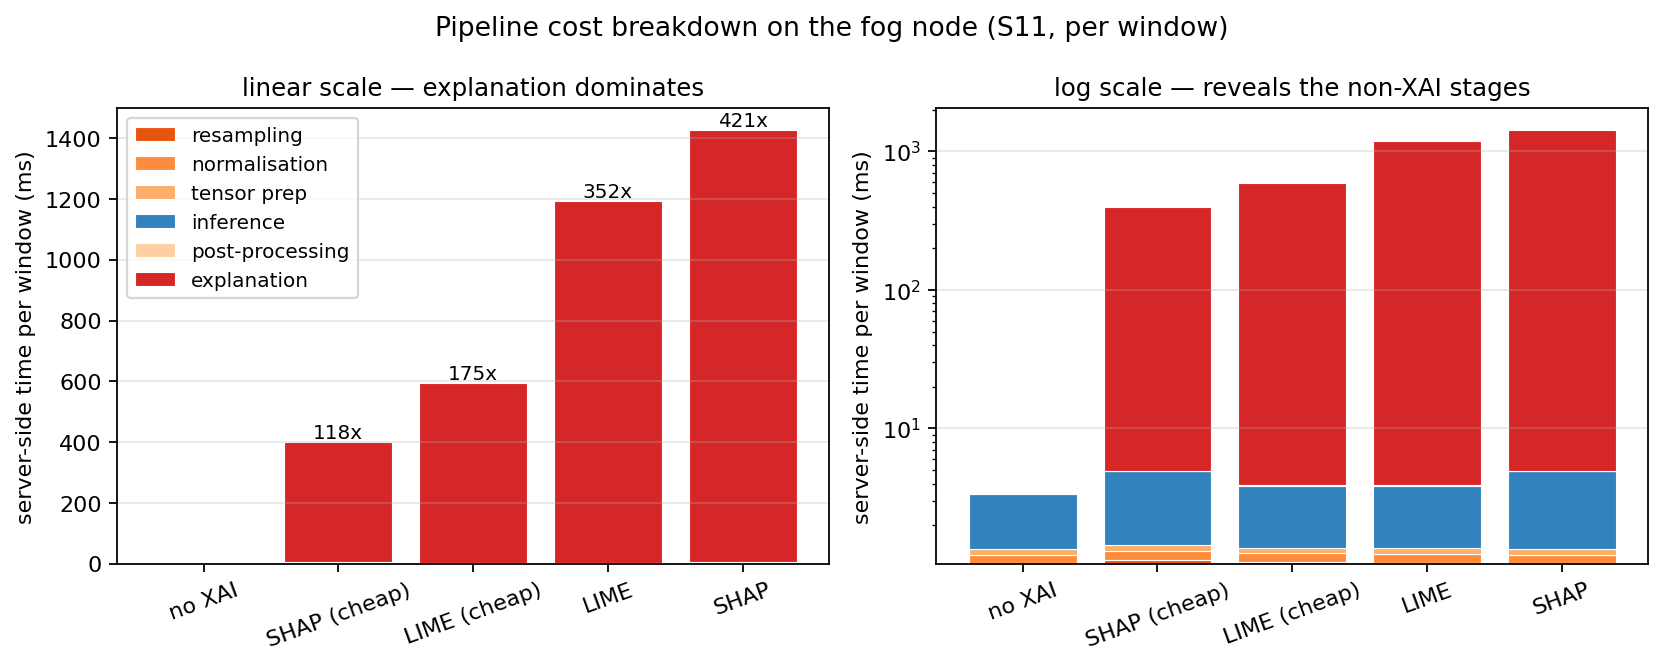
\includegraphics[width=\textwidth]{../results/14_figures/fig1_cost_breakdown.png}
\caption{Sol panel doğrusal ölçekte: açıklama (kırmızı) bütün grafiği
kaplıyor, diğer aşamalar görünmüyor bile. Sağ panel logaritmik ölçekte: aynı
veri, ama yeniden örnekleme (turuncu) ve çıkarım (mavi) artık seçilebiliyor.
Çubukların üstündeki oranlar açıklayıcısız tabana (3{,}39\ms) görelidir.}
\end{figure}

\subsection{Yerleşim kararı, açıklama yükü altında anlamını yitiriyor}

\begin{table}[H]
\centering\small
\begin{tabular}{@{}lrrrr@{}}
\toprule
\textbf{Açıklayıcı} & \textbf{uç (ortak)} & \textbf{sis (LAN)} & \textbf{bulut (internet)} & \textbf{bulut/uç} \\
\midrule
yok               & 7{,}31   & 10{,}62  & \textbf{63{,}52}  & \textbf{8{,}69$\times$} \\
\kod{shap\_cheap} & 462{,}01 & 442{,}61 & 429{,}84 & 0{,}93$\times$ \\
\kod{lime\_cheap} & 352{,}81 & 645{,}22 & 463{,}26 & 1{,}31$\times$ \\
\kod{lime}        & 690{,}05 & 1227{,}54 & 870{,}09 & 1{,}26$\times$ \\
\kod{shap}        & 1154{,}45 & 1456{,}17 & 1300{,}46 & \textbf{1{,}13$\times$} \\
\bottomrule
\end{tabular}
\caption{Üç yerleşim yan yana (medyan yanıt süresi, ms).}
\end{table}

\begin{bulgu}[Raporun en çarpıcı sonucu]
\textbf{Fark ağdan geliyor, hesaptan değil.} Ağ gecikmesi uçta $\approx$1\ms,
siste 4--5\ms, bulutta 40--60\ms. Hesap tarafında bulut VPS'i sis düğümünden
yavaş \emph{değil} --- \kod{shap\_cheap}'te hatta biraz hızlı (337'ye karşı
395\ms) ve bunu \textbf{tek çekirdekle} yapıyor.

Sonuç: XAI'siz durumda bulut, uçtan 8{,}7 kat yavaş; \kod{shap} ile yalnızca
1{,}13 kat --- çünkü 50\ms'lik ağ farkı 1200\ms'lik açıklamanın yanında
kayboluyor. Bu, referans makalenin \emph{``fog, cloud'dan üstündür''}
sonucunu \textbf{XAI yükü altında geçersiz kılıyor}.
\end{bulgu}

\begin{figure}[H]
\centering
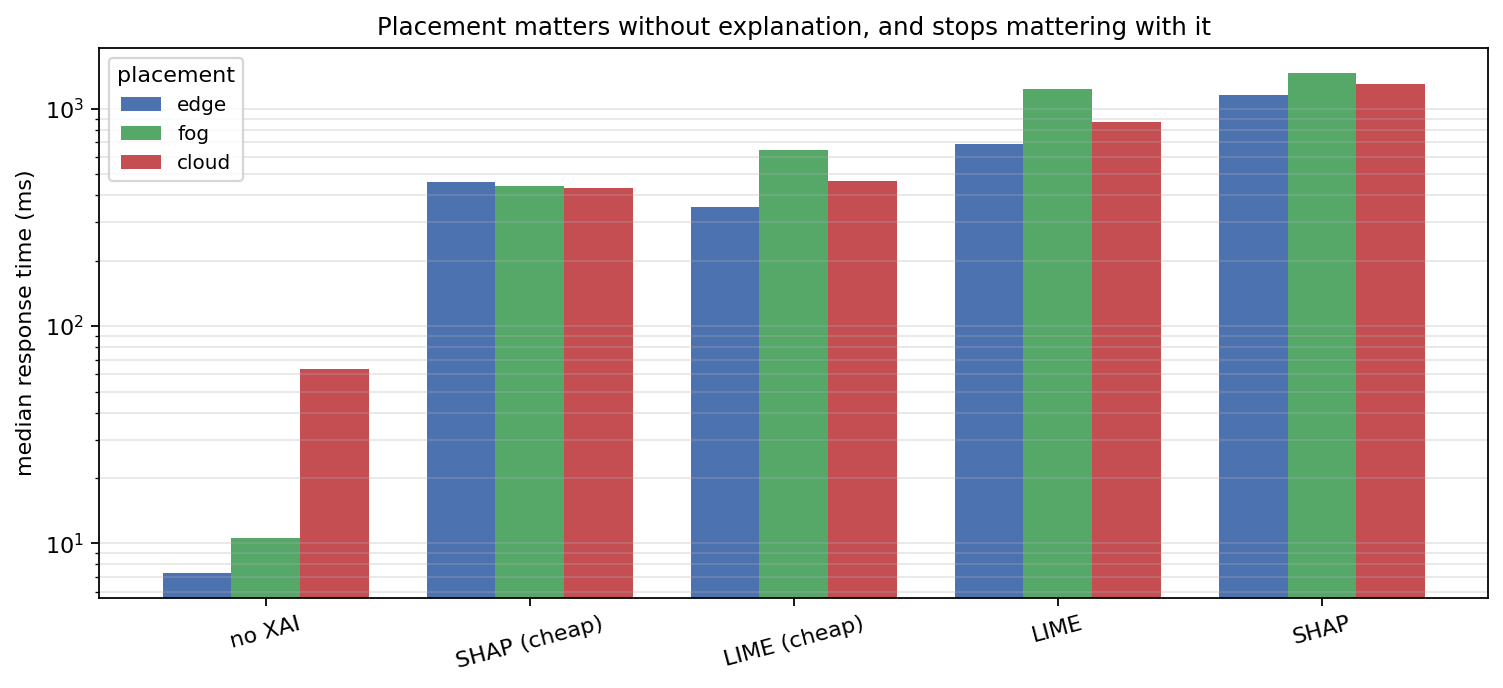
\includegraphics[width=0.92\textwidth]{../results/14_figures/fig5_placement.png}
\caption{Dikey eksen logaritmik. En soldaki grupta üç çubuk arasında büyük
fark var (7 / 11 / 64\ms); sağa doğru, yani açıklama pahalılaştıkça çubuklar
birbirine yaklaşıyor ve en sağda neredeyse eşitleniyor.}
\end{figure}

\subsection{Eşik nasıl seçildi}

Aday eşikler \kod{python -m tools.calibration --tag d1} ile tarandı. Ölçüt:
\emph{düşük \kod{explain\_rate} ile yüksek \kod{error\_recall}}.

\begin{table}[H]
\centering\small
\begin{tabular}{@{}lrrrl@{}}
\toprule
\textbf{eşik} & \textbf{açıklanan} & \textbf{hata yakalama} & \textbf{tetik isabeti} & \textbf{marjinal maliyet} \\
\midrule
0{,}60 & \%6{,}3 (38 pencere) & 0{,}379 (11/29) & 0{,}289 & --- \\
0{,}70 & \%10{,}4 (63) & 0{,}621 (18/29) & 0{,}286 & $+$25 pencere $\to$ $+$7 hata = 3{,}6 \\
\textbf{0{,}80} & \textbf{\%14{,}4 (87)} & \textbf{0{,}897 (26/29)} & \textbf{0{,}299} & $+$24 pencere $\to$ $+$8 hata = \textbf{3{,}0} \\
0{,}90 & \%21{,}4 (129) & 1{,}000 (29/29) & 0{,}225 & $+$42 pencere $\to$ $+$3 hata = \textbf{14{,}0} \\
\bottomrule
\end{tabular}
\caption{S11 (iyi kalibre, 604 pencere, 29 hata).}
\end{table}

\begin{table}[H]
\centering\small
\begin{tabular}{@{}lrrr@{}}
\toprule
\textbf{eşik} & \textbf{açıklanan} & \textbf{hata yakalama} & \textbf{tetik isabeti} \\
\midrule
0{,}60 & \%1{,}7 (10) & 0{,}027 (5/184) & 0{,}500 \\
0{,}70 & \%4{,}4 (26) & 0{,}060 (11/184) & 0{,}423 \\
\textbf{0{,}80} & \textbf{\%11{,}8 (70)} & \textbf{0{,}120 (22/184)} & 0{,}314 \\
0{,}90 & \%29{,}3 (174) & 0{,}288 (53/184) & 0{,}305 \\
\bottomrule
\end{tabular}
\caption{S14 (bozuk kalibre, 594 pencere, 184 hata). Aynı eşikte maliyet
benzer, \emph{fayda} yedi kat düşük.}
\end{table}

\begin{bulgu}[Neden 0{,}80 --- üç gerekçe]
\textbf{1. Eğrinin dirseği orada.} 0{,}60'tan 0{,}80'e kadar her ek hata
$\approx$3 pencereye mal oluyor; 0{,}80'den 0{,}90'a geçişte bu \textbf{14
pencereye} fırlıyor. Son 3 hatayı yakalamak için 42 fazladan açıklama gerekiyor.

\textbf{2. Tetik isabeti 0{,}80'de tepe yapıyor} (0{,}299) ve 0{,}90'da
0{,}225'e çöküyor --- 0{,}90 israf bölgesi.

\textbf{3.} \%86 tasarruf hâlâ duruyor ve hataların \%90'ı yakalanıyor.

Seçim \textbf{elle} yapıldı; otomatik bir ölçüt kullanılmadı.
\end{bulgu}

\textbf{Dört doğrulama koşusu.} Eşik seçildikten sonra sunucuda gerçekten
koşuldu:

\begin{table}[H]
\centering\small
\begin{tabular}{@{}llrrrl@{}}
\toprule
\textbf{\#} & \textbf{Dosya} & \textbf{gerçek eşik} & \textbf{süre} & \textbf{pencere} & \textbf{açıklanan} \\
\midrule
1 & \dosya{kisa\_segment\_sel60.json} & \textbf{0{,}70} & 5 dk & 44 & \textbf{0 (\%0)} \\
2 & \dosya{kisa\_segment\_sel80.json} & 0{,}80 & 5 dk & 44 & \textbf{0 (\%0)} \\
3 & \dosya{kisa\_segment\_sel90.json} & 0{,}90 & 5 dk & 44 & \textbf{0 (\%0)} \\
4 & \textbf{\dosya{fog\_sel80\_tam.json}} & \textbf{0{,}80} & \textbf{87 dk} & \textbf{1030} & \textbf{145 (\%14{,}1)} \\
\bottomrule
\end{tabular}
\end{table}

\begin{uyari}[İlk üç koşu neden \%0 çıktı --- ve dosya adları neden yanıltıcı]
Hata değil, \textbf{kayıt içi durağansızlığın kanıtı}. S11'in ilk 5
dakikasında en düşük güven \textbf{0{,}929}; en yüksek eşik (0{,}90) bile
hiçbir pencerenin altına inmiyor. Düşük güvenli ilk pencere \textbf{\#100},
yani kaydın 8.\ dakikasında; kayıttaki 87 düşük güvenli pencerenin hepsi ilk
400 pencere içinde. Seçici XAI deneyi bu yüzden \textbf{tam kayıt} üzerinde
koşuldu. Bu, ``5 dakikalık örnek yeterlidir'' varsayımının neden tehlikeli
olduğunun somut kanıtıdır.

\textbf{Ayrıca:} \dosya{sel60} gerçekte eşik \textbf{0{,}70} ile koşuldu
(etiket kayması). Gerçek eşikler sunucu künyesinde
(\kod{server.xai.threshold}); \textbf{dosya adına değil künyeye bakılmalı}.
Eşik 0{,}60 hiç koşulmadı.
\end{uyari}

\subsection{Seçici açıklama: ana sonuç}

\begin{table}[H]
\centering\small
\begin{tabular}{@{}lrrrrr@{}}
\toprule
\textbf{Durum} & \textbf{pencere} & \textbf{response ort.} & \textbf{p50} & \textbf{p95} & \textbf{p99} \\
\midrule
hiç açıklama                      & 44 & 15{,}93 & 10{,}62 & 42{,}23 & 91{,}31 \\
\textbf{seçici (0{,}80)}          & \textbf{1030} & \textbf{80{,}13} & \textbf{10{,}95} & \textbf{445{,}70} & 517{,}03 \\
hep açıkla                        & 44 & 450{,}54 & 442{,}61 & 574{,}01 & 599{,}39 \\
\bottomrule
\end{tabular}
\caption{S11 tam kaydı (10\,466 tick, 87 dk), sis düğümü, \kod{shap\_cheap}
(ms). 1030 pencere = diğer sis koşularının 23 katı, yani p95/p99 burada
gerçekten anlamlı. Saat farkı 88 kez yeniden ölçüldü.}
\end{table}

\begin{bulgu}[Ölçülen sonuç]
Seçici açıklama, her pencereyi açıklamaya göre \textbf{5{,}6 kat ucuz}
($450{,}54 / 80{,}13$). Açıklama oranı \%14{,}1 (145/1030); açıklama başına
364{,}82\ms, pencere başına amorti edilmiş 51{,}36\ms. \textbf{Medyan yanıt
süresi 10{,}95\ms} --- tipik pencere, açıklama hiç yokmuş gibi hızlı
cevaplanıyor. Hataların \%89{,}7'si hâlâ açıklanıyor.

\textbf{Kuyrukta birikme YOK:} queuing ortalama 0{,}031\ms, p99 0{,}057\ms.
Patlamalı yükün (\%86 pencere 3{,}6\ms, \%14 pencere $\approx$365\ms) kuyruğu
bozması beklenebilirdi; bozmadı. Sebebi: hop bütçesi 5000\ms{} ve en pahalı
pencere bile 365\ms{} sürüyor, yani bir sonraki pencere gelmeden iş bitiyor.
\end{bulgu}

\begin{table}[H]
\centering\small
\begin{tabular}{@{}lrrr@{}}
\toprule
& \textbf{projeksiyon} & \textbf{ölçüm} & \textbf{hata} \\
\midrule
açıklama oranı    & \%14{,}4 & \%14{,}1 & \textbf{\%2{,}3} \\
ortalama response & 78{,}53\ms & 80{,}13\ms & \textbf{\%2{,}0} \\
p95 response      & 487{,}25\ms & 445{,}70\ms & \%8{,}5 \\
\bottomrule
\end{tabular}
\caption{Karışım modeli ölçümle doğrulandı. Ortalamadaki \%2 beklenen
(karışımın ortalaması matematiksel olarak kesindir); p95'teki \%8{,}5, özet
çeyrekliklerden ara değerle tahmin edildiği için baştan ``yaklaşık'' diye
işaretliydi. \textbf{Sonuç:} dosyadaki diğer 44 satır (öteki açıklayıcılar,
S14) güvenle projeksiyon olarak sunulabilir.}
\end{table}

\begin{figure}[H]
\centering
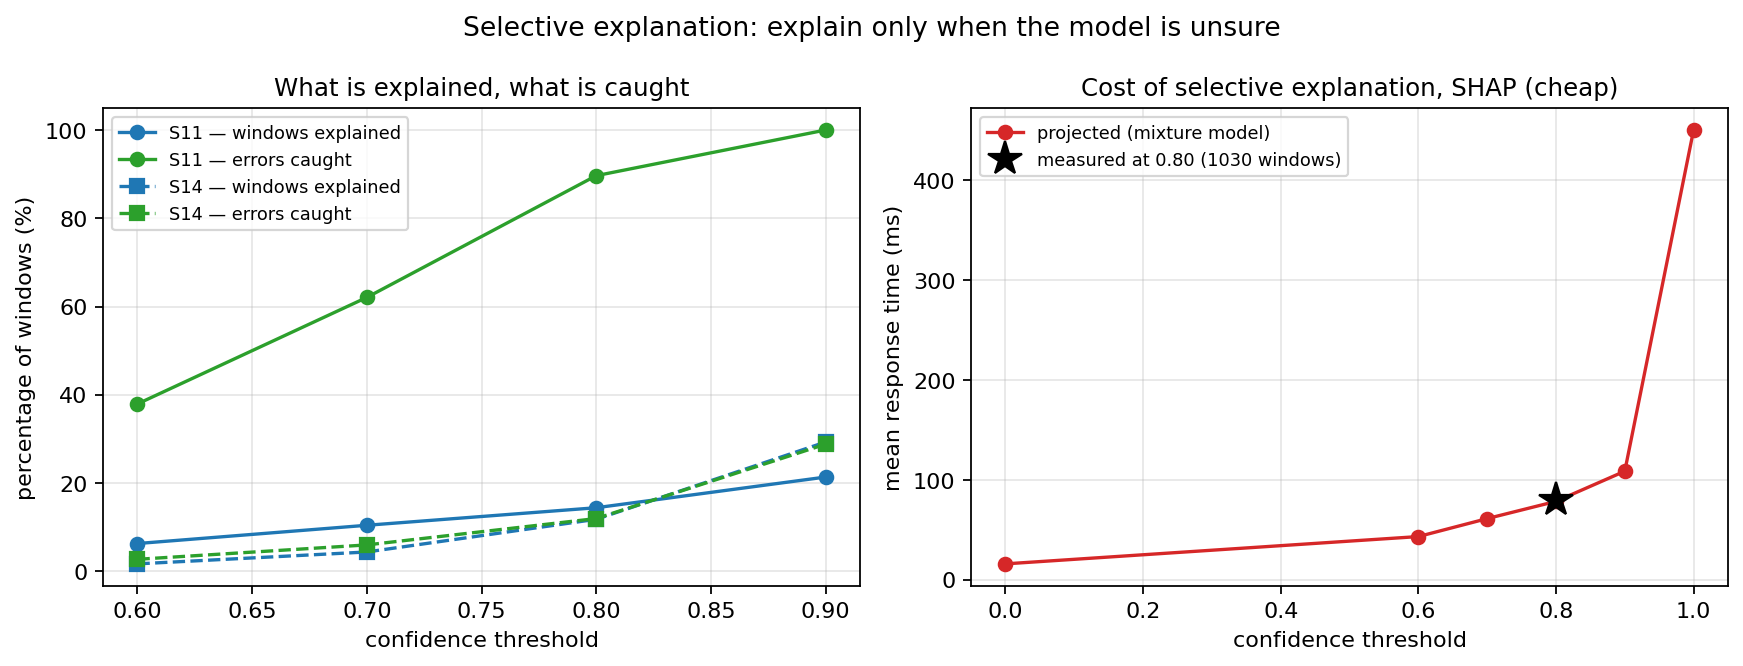
\includegraphics[width=\textwidth]{../results/14_figures/fig2_selective.png}
\caption{Sol panel: eşik yükseldikçe açıklanan pencere oranı (mavi) yavaş,
yakalanan hata oranı (yeşil) hızlı artıyor. S14'te (kesikli) aynı eğri çok
daha düşük --- kalibrasyon bozuk olduğu için hata yakalama \%12'de kalıyor.
Sağ panel: kırmızı eğri karışım modelinin projeksiyonu, siyah yıldız
\textbf{1030 pencerelik gerçek ölçüm}; ikisi üst üste düşüyor.}
\end{figure}

\subsection{Yük altında kapasite}

\begin{table}[H]
\centering\small
\begin{tabular}{@{}llrrrrr@{}}
\toprule
\textbf{Durum} & \textbf{istemci} & \textbf{queuing ort.} & \textbf{q p95} & \textbf{execution} & \textbf{response ort.} & \textbf{p95} \\
\midrule
XAI yok & 1 & 0{,}030 & 0{,}035 & 3{,}59 & 15{,}93 & 42{,}23 \\
XAI yok & 2 & 1{,}607 & 4{,}514 & 3{,}57 & 24{,}31 & 107{,}78 \\
XAI yok & 4 & 4{,}555 & 12{,}505 & 3{,}69 & 28{,}50 & 120{,}27 \\
\midrule
hep açıkla & 1 & 0{,}032 & 0{,}052 & 400{,}18 & 450{,}54 & 574{,}01 \\
hep açıkla & 2 & \textbf{160{,}12} & 381{,}58 & 371{,}06 & 601{,}30 & 853{,}58 \\
hep açıkla & 4 & \textbf{437{,}25} & \textbf{1125{,}11} & 370{,}75 & 984{,}94 & 1643{,}07 \\
\bottomrule
\end{tabular}
\caption{Sis düğümü, \kod{shap\_cheap}, S11+S14 döngüsel, 600 tick (ms).
Bulut karşılığı (4 istemci, XAI yok, 4120 pencere): queuing ort.\ 4{,}74,
p95 16{,}08; response ort.\ 67{,}48, p95 117{,}81\ms.}
\end{table}

\begin{table}[H]
\centering\small
\begin{tabular}{@{}lrr@{}}
\toprule
\textbf{Durum} & \textbf{execution} & \textbf{kapasite (5000/exec)} \\
\midrule
XAI yok         & 3{,}59\ms   & \textbf{1394} istemci \\
seçici (0{,}80) & 55{,}26\ms  & \textbf{90} istemci \\
hep açıkla      & 400{,}18\ms & \textbf{12} istemci \\
\midrule
\multicolumn{2}{@{}l}{\emph{referans makale, tek worker}} & $\approx$20 istemci \\
\bottomrule
\end{tabular}
\caption{Seçici açıklama kapasiteyi \textbf{7{,}5 kat} artırıyor.}
\end{table}

\subsection{Açıklayıcı seçimi: ``daha iyi'' yok, denge var}

\begin{table}[H]
\centering\small
\begin{tabular}{@{}lrrrr@{}}
\toprule
\textbf{Nokta} & \textbf{gecikme} & \textbf{faithfulness $\pm$ SEM} & \textbf{monotonicity} & \textbf{sensitivity $\pm$ SEM} \\
\midrule
\kod{shap\_cheap} & 395\ms  & 0{,}2499 $\pm$ 0{,}0426 & 0{,}5650 & 0{,}1228 $\pm$ 0{,}0032 \\
\kod{lime\_cheap} & 590\ms  & 0{,}2092 $\pm$ 0{,}0345 & 0{,}6038 & \textbf{0{,}0489} $\pm$ 0{,}0016 \\
\kod{lime}        & 1189\ms & 0{,}2324 $\pm$ 0{,}0373 & 0{,}5788 & \textbf{0{,}0446} $\pm$ 0{,}0018 \\
\kod{shap}        & 1422\ms & 0{,}2632 $\pm$ 0{,}0445 & 0{,}5488 & 0{,}1282 $\pm$ 0{,}0046 \\
\bottomrule
\end{tabular}
\caption{S11, 40 pencere. Kaynak: \dosya{11\_pareto/pareto\_c5.json}}
\end{table}

\begin{bulgu}[Üç sonuç]
\textbf{1. Faithfulness'ta hiçbir nokta diğerini yenmiyor} --- dört nokta
0{,}209--0{,}263 aralığında, SEM $\approx$0{,}04, farkların hepsi hata payının
içinde. \emph{Seçim faithfulness'a göre yapılamaz.}

\textbf{2. Ayrışma sensitivity'de ve kesin:} LIME 2{,}7$\times$ daha kararlı,
fark hata payının 15 katı.

\textbf{3. Gerçek denge:} SHAP 3$\times$ ucuz, LIME 2{,}7$\times$ kararlı,
sadakat eşit.

\emph{Örnek başına maliyet tersine dönüyor:} LIME 2{,}4\ms/örnek
($590/250$), SHAP 7{,}9\ms/örnek ($395/50$). Tek örnek düzeyinde SHAP pahalı
--- literatürle uyumlu --- ama çok daha az örnekle yetindiği için toplamda
ucuz. Bu ayrım makalede yazılmalı, yoksa çelişkili görünür.
\end{bulgu}

\subsection{Faydanın koşulu: kalibrasyon}

\begin{table}[H]
\centering\small
\begin{tabular}{@{}lrr@{}}
\toprule
& \textbf{S11} & \textbf{S14} \\
\midrule
pencere / hata sayısı & 604 / 29 & 594 / 184 \\
doğruluk              & \textbf{0{,}9520} & \textbf{0{,}6902} \\
ortalama güven        & 0{,}9093 & 0{,}9085 \\
fazla özgüven         & $-$0{,}0426 & \textbf{$+$0{,}2182} \\
ECE                   & \textbf{0{,}0469} & \textbf{0{,}2265} \\
eşik 0{,}80'de açıklanan & \%14{,}4 & \%11{,}8 \\
eşik 0{,}80'de hata yakalama & \textbf{0{,}897} & \textbf{0{,}120} \\
\bottomrule
\end{tabular}
\caption{İki tutulmuş denek taban tabana zıt.}
\end{table}

\begin{bulgu}[İki iddia ayrı yazılmalı]
Model \textbf{ikisine de aynı güvenle yaklaşıyor} (0{,}909) ama birinde \%95,
diğerinde \%69 haklı. S14'te \emph{kendinden emin biçimde yanılıyor}.

\textbf{Maliyet tasarrufu her iki denekte gerçekleşiyor} (açıklama oranı
\%12--14, kalibrasyondan bağımsız). \textbf{Fayda ise kalibrasyona bağlı}
(hata yakalama \%90'a karşı \%12).

\textbf{Sıcaklık ölçekleme çalışmadı:} çapraz denek uygulaması her iki yönde
de kötüleştirdi (S11 ECE $0{,}047 \rightarrow 0{,}256$; S14
$0{,}227 \rightarrow 0{,}276$). Bozukluk zıt yönlerde olduğu için tek
parametre ikisini birden düzeltemiyor. Bu bir hata değil, raporlanacak bir
bulgudur.
\end{bulgu}

\begin{figure}[H]
\centering
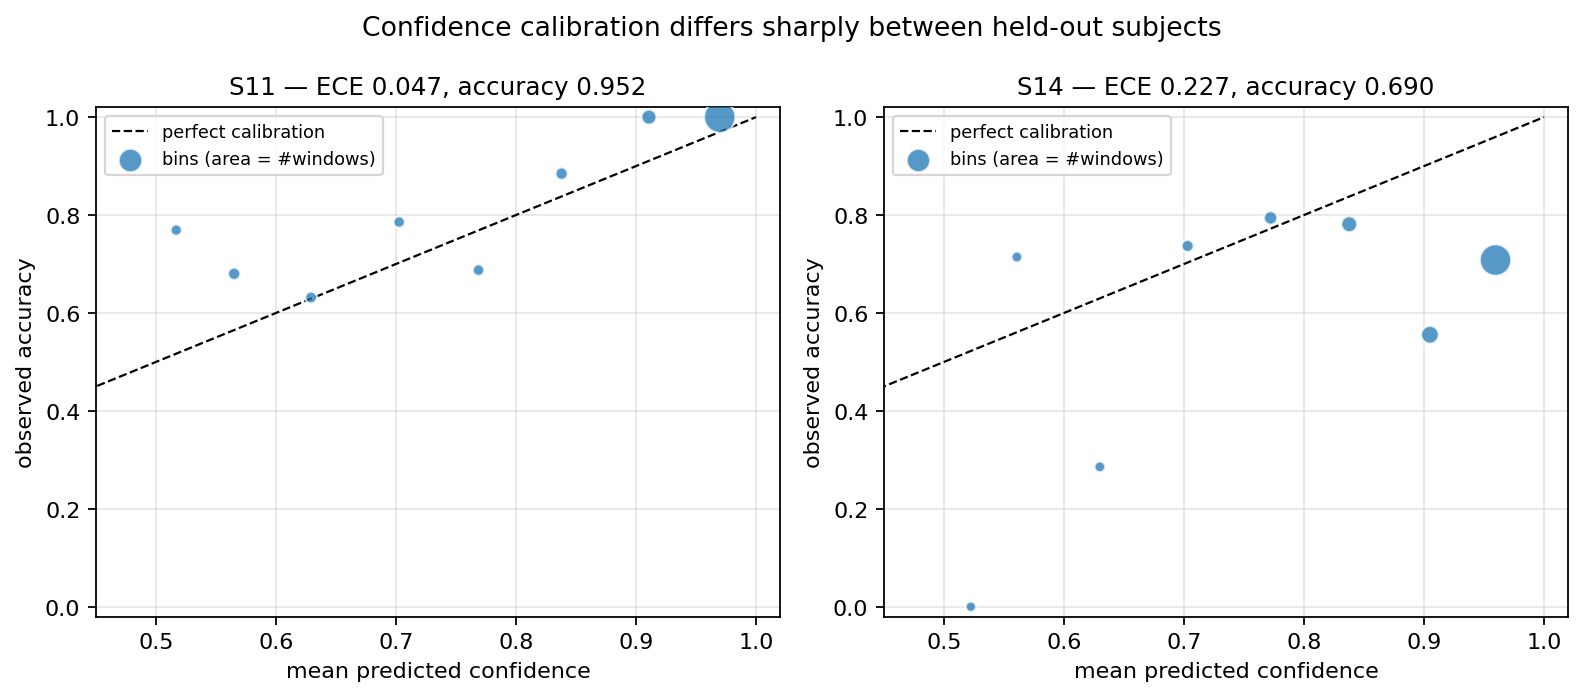
\includegraphics[width=0.95\textwidth]{../results/14_figures/fig6_calibration.png}
\caption{Kesikli köşegen mükemmel kalibrasyon; baloncuk alanı o kutudaki
pencere sayısı. S11 (sol) noktaları köşegenin üstünde veya yakınında. S14
(sağ) en büyük baloncuk köşegenin \emph{altında}: model \%96 güvenle
konuşuyor ama \%71 haklı.}
\label{fig:kal}
\end{figure}

\subsection{Referans makale ile karşılaştırma}

\begin{table}[H]
\centering\small
\begin{tabular}{@{}lrrl@{}}
\toprule
\textbf{Metrik} & \textbf{Makale (worker)} & \textbf{Bu çalışma} & \textbf{Karşılaştırılabilir mi?} \\
\midrule
latency        & 4{,}7\ms  & 0{,}81\ms (loopback) & hayır --- farklı ağ \\
queuing delay  & $<$1\ms   & 0{,}045\ms & hayır \\
execution time & 34{,}7\ms & 7{,}18\ms  & hayır --- Pi 4 vs masaüstü \\
response time  & 43{,}3\ms & 8{,}82\ms  & hayır \\
jitter         & 17{,}4\ms & 3{,}53\ms  & hayır \\
\textbf{bandwidth} & \textbf{374 kbps} & \textbf{187 kbps} & \textbf{evet} \\
\bottomrule
\end{tabular}
\caption{Erzurumluoğlu ve ark., ICACT 2025 (DREAMER, Raspberry Pi 4 worker).}
\end{table}

\begin{bulgu}[Anlamlı olan tek karşılaştırma bant genişliği]
Onlar 3 saniyelik pencereden 24 öznitelik çıkarıp gönderiyor, biz 10 saniyelik
pencerenin \textbf{ham sinyalini} gönderiyoruz --- buna rağmen \textbf{yarısı
kadar} veri geçiyor. Asıl fark mimari: onlarda öznitelik çıkarımı hesabın
çoğunu oluşturuyor, bizde ham sinyal doğrudan modele giriyor.

\textbf{Pi 4 çıkarımı:} referansın Pi 4'ünde execution 34{,}7\ms, bizde
3{,}6\ms{} --- $\approx$10 kat. Aynı oran açıklamaya uygulanırsa
\kod{shap\_cheap} bir Pi 4'te \textbf{$\approx$4 saniye} eder ve 5 saniyelik
hop bütçesini neredeyse doldurur. Yani gerçek sis donanımında seçici açıklama
\emph{zorunlu} hâle gelir.
\end{bulgu}

%=======================================================================
\section{Uyarılar ve sınırlılıklar}

\subsection{Makaleye sayı taşırken dikkat}

\begin{enumerate}[leftmargin=1.5em,itemsep=0.3em]
\item \textbf{Sis XAI koşuları 44 pencere, tek tekrar.} Ortalama
karşılaştırması geçerli; \textbf{p95/p99 yalnızca 1030 pencerelik seçici
koşudan} alınmalı.

\item \textbf{Sis koşularındaki sınıflandırma sayıları anlamsız.} S11'in ilk
5 dakikasında hiç stres etiketi yok (42 pencerenin hepsi stres-olmayan,
doğruluk 1{,}00). Başarım Çizelge~5'ten (Bölüm~4.1) okunmalı.

\item \textbf{Yazılım yığını yerleşimler arasında farklı.} Uç: Python 3.11 /
PyTorch 2.8. Sis: Python 3.14 / PyTorch 2.14. Bulut: Docker python:3.11 /
PyTorch 2.14. Bu yüzden \dosya{07\_edge\_xai} ile \dosya{04\_fog} arasındaki
sıralama tutarsız: LIME'da uç hızlı (390'a karşı 590\ms), SHAP'ın ucuz
noktasında sis hızlı (395'e karşı 417\ms), tabanda sis hızlı. \textbf{Donanım
farkı böyle davranmaz} --- olduğu gibi ``sis daha yavaş'' diye sunulamaz.
Kapatmak için sis düğümünü Docker'la (python:3.11) yeniden koşmak yeterli
($\approx$25 dk).

\item \textbf{Eşik, üzerinde test edildiği denekte seçildi.} $\tau$=0{,}80,
S11'in tablosuna bakılarak seçildi ve ana doğrulama koşusu da S11'de yapıldı.
\dosya{PLAN.md} kural~8 (``eşik seçimi test deneğinde yapılmaz'') bu koşuda
uygulanmadı. S14 için eşik 0{,}80 yalnızca \emph{projeksiyon} olarak var.
Kapatmak için S14 tam kayıt koşusu ($\approx$5 dk) ya da sınırlılıklarda
açık ifade.

\item \textbf{\dosya{results/README.md} ile ham dosyalar arasında beş fark
bulundu.} En önemlisi: \dosya{benchmark\_xai\_cpu.json}'da ``LIME 250 örnek
p50 490\ms'' diye bir kayıt \textbf{yok}; dosyadaki iki kayıt 500 örnek/20
dilim (p50 710\ms) ve 500 örnek/\textbf{5} dilim (p50 678\ms). Ayrıca
\dosya{05\_yerlesim} sayıları farklı (uç 0{,}928 / 6{,}344 / 7{,}880; sis
4{,}910 / 3{,}372 / 10{,}151) ve \dosya{01\_streaming} ``1175 pencere'' değil
2123 ölçülen / 1198 etiketli. Tam liste ayrıntılı raporun 12.\ bölümünde.
\textbf{Makaleye sayı doğrudan JSON'dan okunmalı.}

\item \textbf{\dosya{README.md}'nin ``Ölçülen sonuçlar'' tablosu eski}
(preprocessing 0{,}189\ms, inference 1{,}15\ms, toplam 1{,}27\ms) ---
\kod{prepared} yol dönemine ait.
\end{enumerate}

\subsection{Sınırlılıklar}

\begin{enumerate}[leftmargin=1.5em,itemsep=0.22em]
\item \textbf{İki tutulmuş denek (n=2).} Kalibrasyon bulgusu ve ``denek
bağımlı'' sonucu genelleme değil, gözlemdir.
\item \textbf{Sis düğümü bir masaüstü, Raspberry Pi değil.} Ölçülen şey
\emph{dağıtık yerleşim}, \emph{kaynak kısıtlı sis düğümü} değil. Tek çekirdeğe
kilitlemenin bu iş yükünde hiçbir şey değiştirmediği ölçüldü (süreç zaten tek
iplik, tepe CPU \%105--111); bağlayıcı tek yöntem kesirli CPU kotasıdır
(Docker \kod{--cpus=0.1}).
\item \textbf{Kuyruk ölçümü bir üst sınırdır} (istemciler faz hizalı başlıyor).
\item \textbf{Latency Wi-Fi ve internette belirsiz} ($\pm$1--1{,}7\ms{} /
$\pm$25--51\ms). Execution, queuing, response ve jitter bundan etkilenmez.
\item \textbf{Emülasyon, canlı sistem değil.} WESAD kaydından replay yapılıyor
--- referans makalenin de yaptığı budur, ama ``clinical'' veya ``live system''
denmemeli.
\item \textbf{Tek model, iki açıklayıcı}; kullanıcı çalışması yok; MCU analizi
kâğıt üstünde.
\end{enumerate}

%=======================================================================
\section{Kaynak haritası ve komutlar}

\begin{table}[H]
\centering\footnotesize
\begin{tabular}{@{}p{6.1cm}p{8.5cm}@{}}
\toprule
\textbf{Sonuç} & \textbf{Kaynak} \\
\midrule
Aşama bazlı hesaplama profili & \dosya{01\_streaming/streaming\_summary\_native\_fixed.json} \\
İplik / ardışık düzen taraması & \dosya{02\_benchmark/benchmark\_thread\_sweep.json},\newline \dosya{benchmark\_pipeline\_cmp.json} \\
Açıklayıcıların istemci CPU maliyeti & \dosya{02\_benchmark/benchmark\_xai\_cpu.json} \\
Yedi metrik, loopback & \dosya{03\_loopback/fog\_realtime\_1user.json} \\
\textbf{Ana maliyet tablosu} & \dosya{04\_fog/fog\_xai\_*.json} \\
Uç vs sis (XAI'siz) & \dosya{05\_yerlesim/deployments\_edge\_vs\_fog.json} \\
XAI hiperparametre taraması & \dosya{06\_xai\_tarama/*.csv} \\
Ortak yerleşimde XAI & \dosya{07\_edge\_xai/edge\_xai\_*.json} \\
Kalibrasyon, ECE, eşik tablosu & \dosya{08\_kalibrasyon/calibration\_d1.json} \\
\textbf{Seçici açıklama, ana koşu} & \dosya{09\_secici\_xai/fog\_sel80\_tam.json} \\
Eşik projeksiyonu (48 satır) & \dosya{09\_secici\_xai/selective\_xai\_sweep\_d2.json} \\
Çok istemcili yük ve kapasite & \dosya{10\_yuk/fog\_load\_*.json} \\
Kalite--gecikme Pareto & \dosya{11\_pareto/pareto\_c5.json} \\
Aşama profili derlemesi & \dosya{12\_profil/profile\_table\_b1.json} \\
Bulut yerleşimi & \dosya{13\_bulut/cloud\_*.json} \\
Şekiller & \dosya{14\_figures/} (\kod{python -m tools.figures}) \\
Seçilmiş XAI yapılandırmaları & \dosya{checkpoints/xai\_config.json} \\
SHAP arka plan kümesi & \dosya{checkpoints/shap\_background\_k100\_kmeans.npz} \\
Geçersiz sayılan ölçümler & \dosya{results/eski\_ve\_hatali/} (+ kendi README'si) \\
\bottomrule
\end{tabular}
\end{table}

\begin{tcolorbox}[colback=acikGri,colframe=black!30,boxrule=0.6pt,breakable]
\ttfamily\footnotesize
\# Sunucuyu ikinci makinede başlat (seçici XAI ile)\\
python -m serving.server --host 0.0.0.0 --port 9099 \textbackslash\\
\hspace*{2em}--xai-method shap\_cheap --xai-threshold 0.8\\[0.4em]
\# İstemci (verinin olduğu makinede)\\
python run\_fog\_experiment.py --server-host 192.168.1.14 \textbackslash\\
\hspace*{2em}--subject S11 --realtime --tag sel80\_tam\\[0.4em]
\# Yerleşim karşılaştırması (dönüşümlü, 3 tekrar)\\
python compare\_deployments.py --subject S11 --realtime --max-ticks 600 \textbackslash\\
\hspace*{2em}--repeat 3 --deployment edge=local fog=192.168.1.14 --tag edge\_vs\_fog\\[0.4em]
\# Tekrarlı, dönüşümlü profil ölçümü\\
python benchmark\_runs.py --subject S11 --repeat 4 --threads 1 2 4 --tag thread\_sweep\\[0.4em]
\# Türetilmiş çıktılar\\
python -m tools.calibration --tag d1\\
python -m tools.selective\_sweep --tag d2\\
python -m tools.pareto --tag c5\\
python -m tools.profile\_table\\
python -m tools.figures\\
python -m tools.mcu\_feasibility\\[0.4em]
\# Docker ile bulut dağıtımı (sunucu WESAD verisine ihtiyaç duymaz)\\
WESAD\_XAI\_METHOD=shap\_cheap WESAD\_XAI\_THRESHOLD=0.8 docker compose up -d --build
\end{tcolorbox}

\vspace{0.5em}
\begin{center}\small
\textit{Ayrıntılı sürüm:} \dosya{docs/teknik\_rapor.pdf} --- tam sözlük,
13 deneyin tek tek dökümü, geçersiz sayılan ölçümlerin gerekçeleri,
bitirme projesi sonuçları ve tespit edilen tutarsızlıkların tam listesi.
\end{center}

\end{document}
